\documentclass{praktikum}
\usepackage{graphicx}
\usepackage{caption}
\usepackage{subcaption}
\graphicspath{ {./} }
\usepackage{pgfplotstable}
%====== Vyplňte údaje ======
%% dobrá rada na začátek - pokud nevíš, co měníš, zálohuj to, co funguje ;)

\jmeno{Matyáš Peroutík}
\kod{256371}
\rocnik{1}
\obor{AMT}
\skupina{}
\labskup{B}
\spolupracoval{Štěpán Pavlica}


\ucitel{}
\merenodne{10.\,04.\,2024}
\odevzdanodne{07.\,04.\,2024}

\priprava{}
\opravy{}
\nazev{Měrný náboj elektronu}
\cislo{25} %měřené úlohy

\usepackage{fancyhdr}
\usepackage{lastpage}
\pagestyle{fancy}
\fancyhf{}
\renewcommand{\headrulewidth}{0pt}
 
\rfoot{Strana \thepage \hspace{1pt} z \pageref{LastPage}}

\begin{document}

%====== Vygenerování tabulky ======
\maketitle
\vspace{0.5 cm}

%====== Text protokolu zde ======

\section{Úkol měření}
\paragraph{}Stanovte měrný náboj elektronu $\dfrac{e}{m}$ a výsledek porovnejte s tabulkovou hodnotou.
\section{Teoretický rozbor}
\paragraph{}
Magnetron je vakuová dioda s katodou a anodou ve tvaru souosých válců, která je umístěna v homogenním magnetickém poli. Magnetické pole způsobí zakřivení dráhy elektronů. To se projeví snížením proudu diodou. Mezi elektrodami je napětí $U_a$. Velikost homogenního magnetického pole vypočteme podle vztahu:

\begin{equation}
\label{eqn:mag_pole_civkou}
B = \mu _0 \frac{N}{L}I_c
\end{equation}$I_c$ \dotfill Magnetizační proud procházející cívkou\\
N \dotfill Počet závitů cívky \\
L \dotfill Délka cívky \\
$\mu _0$ \dotfill Absolutní permeabilita vakua ($4\pi 10^{-7}$) \\

Pokud zanedbáme deformaci mag. pole na koncích cívky a deformaci elektrického pole na konci koaxiálního uspořádání elektrod, můžeme pro elektrickou a magnetickou sílu působící na elektron použít následující vztahy:

\begin{equation}
\label{eqn:sila_elektrickeho_pole}
F_e = eE
\end{equation}

\begin{equation}
\label{eqn:sila_magnetickeho_pole}
F_m = eBv
\end{equation}

Jelikož je elektron záporně nabitá částice, tak síla $\vec{F_e}$ má radiální směr od katody k anodě. Směr působení magnetického pole, který je dán následujícím vztahem, je v každém okamžiku kolmý na rychlost $\vec{v}$, což má za důsledek zakřivení dráhy.

\begin{equation}
\vec{F_m} = e\vec{v}\times\vec{B}
\end{equation}

Pokud budeme uvažovat, že elektrony mají při výstupu z katody nulovou počáteční rychlost, že válcové plochy jsou nekonečně dlouhé, a označíme li poloměr anody $R_a$, její potenciál $U_a$ a obdobné označení pro katodu, budou síly, kterými na ně pole působí, ležet v rovině kolmé k ose válcových elektrod. \hfill \\

\indent Dráhu elektronu v magnetickém a elektrickém poli popisuje následující pohybová rovnice:

\begin{equation}
\label{eqn:pohybovka_elektronu}
m\vec{a}=\sum\vec{F}=\vec{F_e}+\vec{F_m}
\end{equation}

Po dosazení za veličiny dostaneme následující vztah:

\begin{equation}
\label{eqn:upravena_pohybovka_elektronu}
m\frac{d^2\vec{r}(t)}{dt^2}=e\vec{E}+e(\vec{v}\times\vec{B})
\end{equation}m\dotfill Hmotnost elektronu\\
e\dotfill Náboj elektronu\\
$\vec{r}(t)$\dotfill Polohový vektor elektronu v čase t\\
$\vec{v}$\dotfill Vektor okamžité rychlosti elektronu\\
$\vec{E}$\dotfill Vektor intenzity elektrického pole\\
$\vec{B}$ \dotfill Vektor magnetické indukce\\

\indent Pokud chceme zjistit kritickou velikost magnetické indukce, při které dochází změně řešení pohybové rovnice (\ref{eqn:upravena_pohybovka_elektronu}) z cykloidy na krmužnici, budeme předpokládat, že se takto bude většina elektronů pohybovat. Pro pohyb částice v uzavřené soustavě po kruhové dráze poté platí, že její moment hybnosti b je konstantní. V tomto uspořádání se dá vypočítat následovně:
\begin{equation}
\label{eqn:moment_hybnosti}
b=mr^2\frac{d\varphi}{dt}+\frac{1}{2}er^2B=konst.
\end{equation}$\dfrac{d\varphi}{dt}=\omega$\dotfill Úhlová rychlost elektronu\\
r\dotfill Poloměr dráhy elektronu\\


Pro dva velmi blízké kruhové dráty dostaneme pro úhlovou rychlost následující vztah:

\begin{equation}
\label{eqn:uhlova_rychlost_2draty}
\dfrac{d\varphi}{dt}=\dfrac{1}{2}\dfrac{e}{m}B
\end{equation}

Energetickou bilanci pro elektron, který vyletěl z katody velice malou počáteční rychlostí do elektrického pole, které mu přídává kinetickou energii určenou napětím $U_a$ můžeme vyjádřit následující rovnicí
\begin{equation}
\label{eqn:energeticka_bilance}
\dfrac{1}{2}m(R_a^2-R_k^2)^2\left(\dfrac{d\varphi}{dt}\right)^2=eU_a
\end{equation}
\indent Po dosazení (\ref{eqn:uhlova_rychlost_2draty}) do (\ref{eqn:energeticka_bilance}) dostaneme nasledující vztah:
\begin{equation}
\label{eqn:energeticka_bilance_dosazeni}
\dfrac{1}{2}m(R_a^2-R_k^2)^2\left(\dfrac{1}{2}\dfrac{eB_0}{m}\right)^2=eU_a
\end{equation}

Z této rovnice můžeme vyjádřit vztah pro měrný náboj elektronu
\begin{equation}
\label{eqn:merny_naboj}
\dfrac{e}{m}=\dfrac{8U_AR_a^2}{\left(R_a^2-R_k^2\right)^2B_0^2}
\end{equation}

\section{Schéma zapojení}
\begin{figure}[H]
\centering
\caption{Schéma zapojení úlohy}
\label{img:schema}
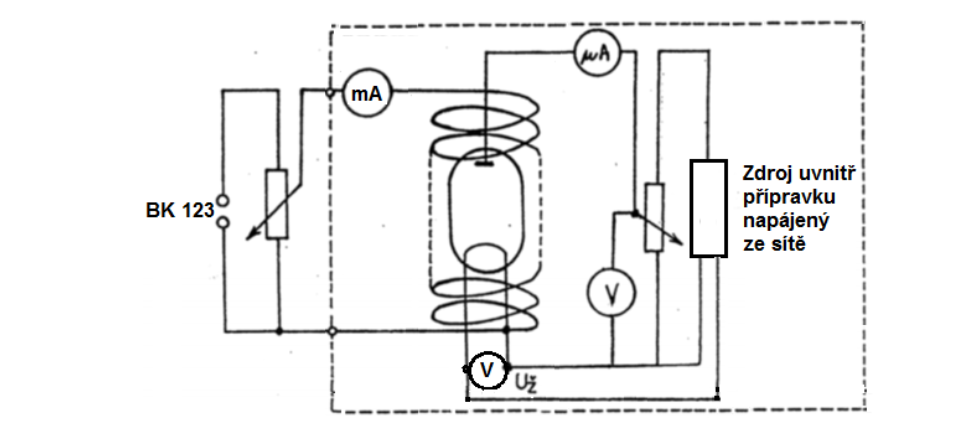
\includegraphics[width=0.7\textwidth]{schema}
\end{figure}

\section{Zpracování naměřených hodnot}
% Please add the following required packages to your document preamble:
% \usepackage{graphicx}
\begin{table}[H]
\centering
\resizebox{0.5\columnwidth}{!}{%
\begin{tabular}{|cc|cc|cc|}
\hline
\multicolumn{2}{|c|}{\textit{\textbf{Ua = 8V}}}     & \multicolumn{2}{c|}{\textit{\textbf{Ua = 10V}}}    & \multicolumn{2}{c|}{\textit{\textbf{Ua = 12V}}}    \\ \hline
\multicolumn{1}{|c|}{\textbf{Ic}}   & \textbf{Ia}   & \multicolumn{1}{c|}{\textbf{Ic}}   & \textbf{Ia}   & \multicolumn{1}{c|}{\textbf{Ic}}   & \textbf{Ia}   \\ \hline
\multicolumn{1}{|c|}{\textit{(mA)}} & \textit{(uA)} & \multicolumn{1}{c|}{\textit{(mA)}} & \textit{(uA)} & \multicolumn{1}{c|}{\textit{(mA)}} & \textit{(uA)} \\ \hline
\multicolumn{1}{|c|}{0}   & 35 & \multicolumn{1}{c|}{0}   & 40 & \multicolumn{1}{c|}{0}   & 46 \\ \hline
\multicolumn{1}{|c|}{30}  & 36 & \multicolumn{1}{c|}{30}  & 40 & \multicolumn{1}{c|}{30}  & 46 \\ \hline
\multicolumn{1}{|c|}{60}  & 36 & \multicolumn{1}{c|}{60}  & 40 & \multicolumn{1}{c|}{60}  & 46 \\ \hline
\multicolumn{1}{|c|}{90}  & 36 & \multicolumn{1}{c|}{90}  & 40 & \multicolumn{1}{c|}{90}  & 45 \\ \hline
\multicolumn{1}{|c|}{120} & 36 & \multicolumn{1}{c|}{120} & 39 & \multicolumn{1}{c|}{120} & 43 \\ \hline
\multicolumn{1}{|c|}{150} & 35 & \multicolumn{1}{c|}{150} & 38 & \multicolumn{1}{c|}{150} & 42 \\ \hline
\multicolumn{1}{|c|}{180} & 34 & \multicolumn{1}{c|}{180} & 37 & \multicolumn{1}{c|}{180} & 42 \\ \hline
\multicolumn{1}{|c|}{210} & 33 & \multicolumn{1}{c|}{210} & 36 & \multicolumn{1}{c|}{210} & 41 \\ \hline
\multicolumn{1}{|c|}{240} & 32 & \multicolumn{1}{c|}{240} & 34 & \multicolumn{1}{c|}{240} & 40 \\ \hline
\multicolumn{1}{|c|}{270} & 31 & \multicolumn{1}{c|}{270} & 31 & \multicolumn{1}{c|}{270} & 39 \\ \hline
\multicolumn{1}{|c|}{300} & 30 & \multicolumn{1}{c|}{300} & 30 & \multicolumn{1}{c|}{300} & 38 \\ \hline
\multicolumn{1}{|c|}{330} & 30 & \multicolumn{1}{c|}{330} & 28 & \multicolumn{1}{c|}{330} & 36 \\ \hline
\multicolumn{1}{|c|}{360} & 28 & \multicolumn{1}{c|}{360} & 25 & \multicolumn{1}{c|}{360} & 33 \\ \hline
\multicolumn{1}{|c|}{390} & 26 & \multicolumn{1}{c|}{390} & 20 & \multicolumn{1}{c|}{390} & 32 \\ \hline
\multicolumn{1}{|c|}{420} & 23 & \multicolumn{1}{c|}{420} & 16 & \multicolumn{1}{c|}{420} & 29 \\ \hline
\multicolumn{1}{|c|}{450} & 20 & \multicolumn{1}{c|}{450} & 13 & \multicolumn{1}{c|}{450} & 26 \\ \hline
\multicolumn{1}{|c|}{480} & 16 & \multicolumn{1}{c|}{480} & 10 & \multicolumn{1}{c|}{480} & 22 \\ \hline
\multicolumn{1}{|c|}{510} & 15 & \multicolumn{1}{c|}{510} & 7  & \multicolumn{1}{c|}{510} & 20 \\ \hline
\multicolumn{1}{|c|}{540} & 12 & \multicolumn{1}{c|}{540} & -  & \multicolumn{1}{c|}{540} & 16 \\ \hline
\multicolumn{1}{|c|}{570} & 9  & \multicolumn{1}{c|}{570} & -  & \multicolumn{1}{c|}{570} & 13 \\ \hline
\multicolumn{1}{|c|}{600} & 7  & \multicolumn{1}{c|}{600} & -  & \multicolumn{1}{c|}{600} & 12 \\ \hline
\multicolumn{1}{|c|}{630} & 6  & \multicolumn{1}{c|}{630} & -  & \multicolumn{1}{c|}{630} & 10 \\ \hline
\multicolumn{1}{|c|}{660} & 5  & \multicolumn{1}{c|}{660} & -  & \multicolumn{1}{c|}{660} & 8  \\ \hline
\end{tabular}%
}
\caption{Naměřené hodnoty}
\label{tab:namerene_hodnoty}
\end{table}
% Please add the following required packages to your document preamble:
% \usepackage{graphicx}
\begin{table}[H]
\centering
\resizebox{0.8\columnwidth}{!}{%
\begin{tabular}{|lc|l|lc|}
\hline
\multicolumn{2}{|c|}{\textbf{Parametry cívky}}          &  & \multicolumn{2}{c|}{\textbf{Parametry elektronky}} \\ \hline
\multicolumn{1}{|l|}{délka / mm}   & \textit{325}  &  & \multicolumn{1}{l|}{poloměr katody / mm} & 3                     \\ \hline
\multicolumn{1}{|l|}{počet závitů} & \textit{5580} &  & \multicolumn{1}{l|}{poloměr anody / mm}  & 5 \\ \hline
\multicolumn{1}{|l|}{průměr vodiče / mm} & \textit{0.6} &  & \multicolumn{1}{l|}{žhavící napětí / V}   & 6.04   \\ \hline
\multicolumn{1}{|l|}{počet vrstev} & \textit{9}    &  & \multicolumn{1}{l|}{}                    & \multicolumn{1}{l|}{} \\ \hline
\end{tabular}%
}
\caption{Parametry měřených prvků}
\label{tab:parametry}
\end{table}

\indent Hodnoty z této tabulky poté převedeme do grafů. Pokud grafy proložíme přímkou, kterou vytvoříme pomocí metody nejmenších čtverců z lineární části měření, dostaneme v průsečíku s maximem hodnotu kritického proudu.



\subsection{Grafy}
\begin{figure}[H] \centering

    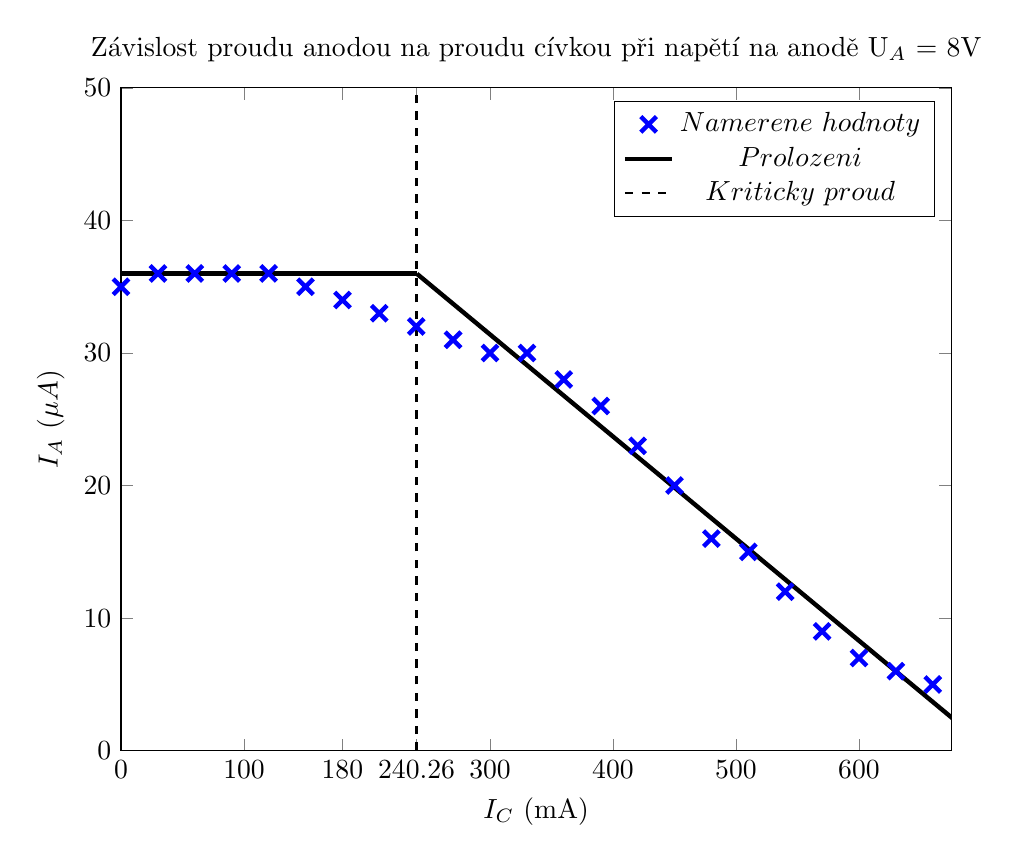
\begin{tikzpicture}[]
\begin{axis}[
    title={Závislost proudu anodou na proudu cívkou při napětí na anodě U$_A$ = 8V},
    xlabel={$I_C$ (mA)},
    ylabel={$I_A$ ($\mu A$)},
    xmin=0, xmax=675,
    ymin=0, ymax=50,
    width = \textwidth,
    height = 10cm,
    xtick={0, 100, 180, 240.26, 300, 400, 500, 600},
]
 
\addplot[
    color=blue,
    mark=x, mark size=4pt,
    ultra thick,
    only marks,
    ]
    coordinates {
    (0, 35)
    (30, 36)
    (60, 36)
    (90, 36)
    (120, 36)
    (150, 35)
    (180, 34)
    (210, 33)
    (240, 32)
    (270,31)
    (300, 30)
    (330, 30)
    (360, 28)
    (390, 26)
    (420, 23)
    (450, 20)
    (480, 16)
    (510, 15)
    (540, 12)
    (570,9)
    (600, 7)    
	(630, 6)
	(660, 5)
    };
    \addlegendentry{$Namerene~hodnoty$}

\addplot[
domain=240.6:700, 
    samples=100,
    color=black,
    ultra thick,
    ]
    {-0.077*x + 54.5};
    \addplot[
    color=black,
    thick, dashed
    ]
    coordinates {
    (240.26, 0)
    (240.26, 100)};
\addplot[
domain=0:240.6, 
    samples=100,
    color=black,
    ultra thick,
    ]
    {36};
       \addlegendentry{$Prolozeni$}

    

    \addlegendentry{$Kriticky~proud$}

\end{axis}
\end{tikzpicture}
\end{figure}


\begin{figure}[H] \centering

    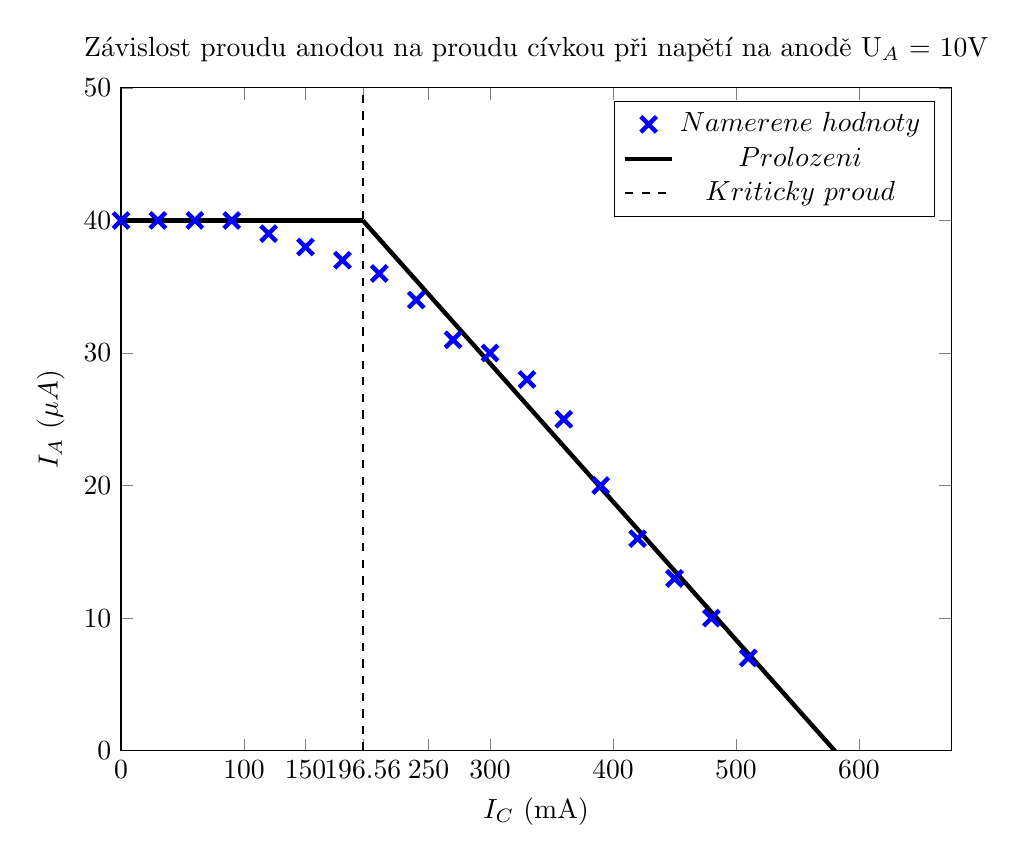
\begin{tikzpicture}[]
\begin{axis}[
    title={Závislost proudu anodou na proudu cívkou při napětí na anodě U$_A$ = 10V},
    xlabel={$I_C$ (mA)},
    ylabel={$I_A$ ($\mu A$)},
    xmin=0, xmax=675,
    ymin=0, ymax=50,
    width = \textwidth,
    height = 10cm,
    xtick={0, 100,150, 196.56, 250,300, 400, 500, 600},
]
 
\addplot[
    color=blue,
    mark=x,mark size=4pt,
    ultra thick,
    only marks,
    ]
    coordinates {
    (0, 40)
    (30, 40)
    (60, 40)
    (90, 40)
    (120, 39)
    (150, 38)
    (180, 37)
    (210, 36)
    (240, 34)
    (270,31)
    (300, 30)
    (330, 28)
    (360, 25)
    (390, 20)
    (420, 16)
    (450, 13)
    (480, 10)
    (510, 7)
    };
    \addlegendentry{$Namerene~hodnoty$}

\addplot[
domain=196.56:660, 
    samples=100,
    color=black,
    ultra thick,
    ]
    {-0.10424242*x + 60.49};
    \addplot[
    color=black,
    thick, dashed
    ]
    coordinates {
    (196.56, 0)
    (196.56, 100)};
\addplot[
domain=0:196.56, 
    samples=100,
    color=black,
    ultra thick,
    ]
    {40};
       \addlegendentry{$Prolozeni$}

    

    \addlegendentry{$Kriticky~proud$}

\end{axis}
\end{tikzpicture}
\end{figure}


\begin{figure}[H] \centering

    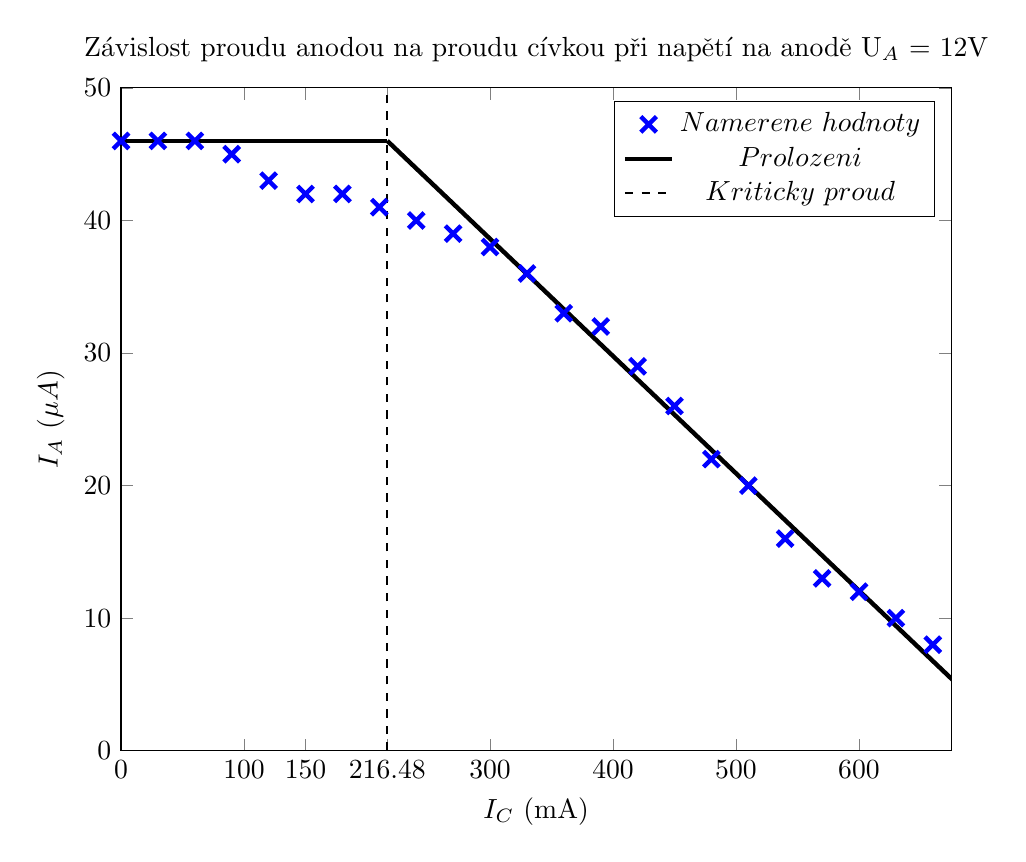
\begin{tikzpicture}[]
\begin{axis}[
    title={Závislost proudu anodou na proudu cívkou při napětí na anodě U$_A$ = 12V},
    xlabel={$I_C$ (mA)},
    ylabel={$I_A$ ($\mu A$)},
    xmin=0, xmax=675,
    ymin=0, ymax=50,
    width = \textwidth,
    height = 10cm,
    xtick={0, 100, 150, 216.48, 300, 400, 500, 600},
]
 
\addplot[
    color=blue,
    mark=x, mark size=4pt,
    ultra thick,
    only marks,
    ]
    coordinates {
    (0, 46)
    (30, 46)
    (60, 46)
    (90, 45)
    (120, 43)
    (150, 42)
    (180, 42)
    (210, 41)
    (240, 40)
    (270,39)
    (300, 38)
    (330, 36)
    (360, 33)
    (390, 32)
    (420, 29)
    (450, 26)
    (480, 22)
    (510, 20)
    (540, 16)
    (570,13)
    (600, 12)    
	(630, 10)
	(660, 8)
    };
    \addlegendentry{$Namerene~hodnoty$}

\addplot[
domain=216.48:700, 
    samples=100,
    color=black,
    ultra thick,
    ]
    {-0.08846*x + 65.153846};
    \addplot[
    color=black,
    thick, dashed
    ]
    coordinates {
    (216.48, 0)
    (216.48, 100)};
\addplot[
domain=0:216.48, 
    samples=100,
    color=black,
    ultra thick,
    ]
    {46};
       \addlegendentry{$Prolozeni$}

    

    \addlegendentry{$Kriticky~proud$}


\end{axis}
\end{tikzpicture}
\end{figure}

\begin{figure}[H] \centering

    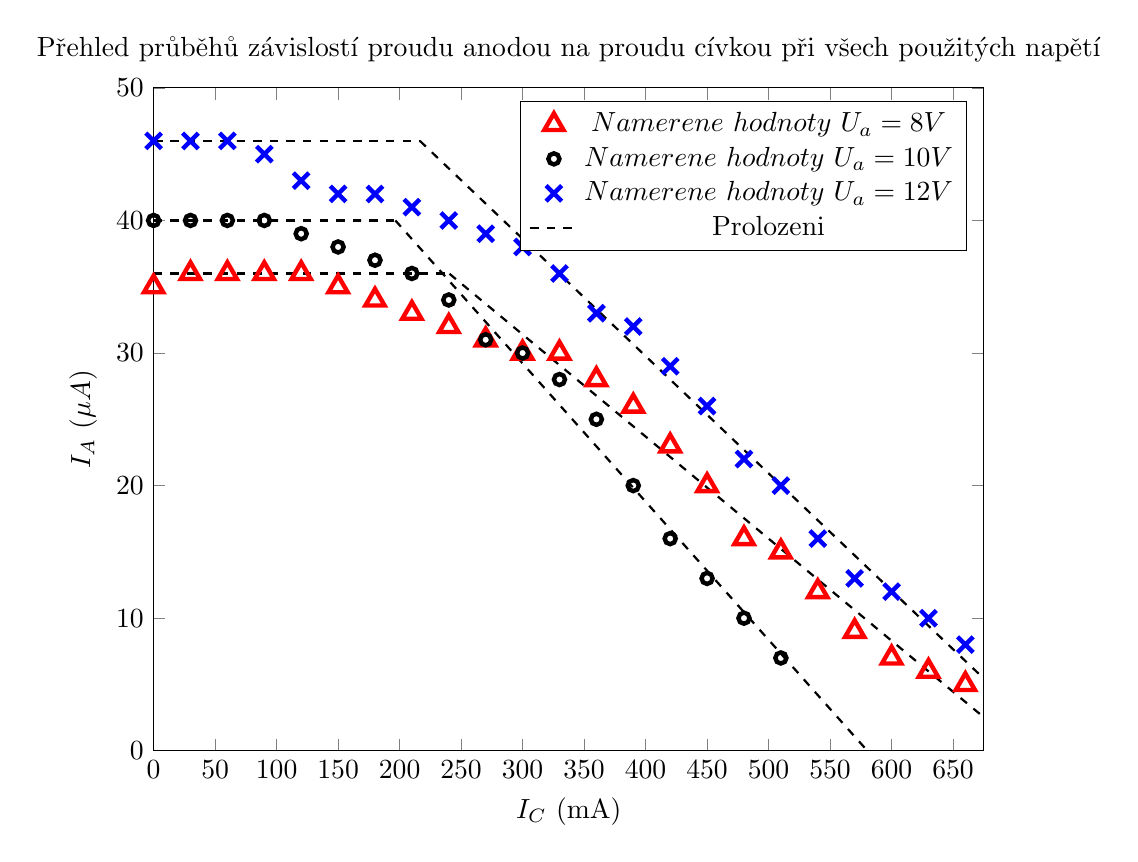
\begin{tikzpicture}[]
\begin{axis}[
    title={Přehled průběhů závislostí proudu anodou na proudu cívkou při všech použitých napětí},
    xlabel={$I_C$ (mA)},
    ylabel={$I_A$ ($\mu A$)},
    xmin=0, xmax=675,
    ymin=0, ymax=50,
    width = \textwidth,
    height = 10cm,
    xtick={0, 50, 100, 150, 200,250, 300,350,  400,450, 500,550, 600, 650},
]

\addplot[
    color=red,
    mark=triangle, mark size=4pt,
    ultra thick,
    only marks,
    ]
    coordinates {
    (0, 35)
    (30, 36)
    (60, 36)
    (90, 36)
    (120, 36)
    (150, 35)
    (180, 34)
    (210, 33)
    (240, 32)
    (270,31)
    (300, 30)
    (330, 30)
    (360, 28)
    (390, 26)
    (420, 23)
    (450, 20)
    (480, 16)
    (510, 15)
    (540, 12)
    (570,9)
    (600, 7)    
	(630, 6)
	(660, 5)
    };
 \addplot[
    color=black,
    mark=o,
    ultra thick,
    only marks,
    ]
    coordinates {
    (0, 40)
    (30, 40)
    (60, 40)
    (90, 40)
    (120, 39)
    (150, 38)
    (180, 37)
    (210, 36)
    (240, 34)
    (270,31)
    (300, 30)
    (330, 28)
    (360, 25)
    (390, 20)
    (420, 16)
    (450, 13)
    (480, 10)
    (510, 7)
    };
\addplot[
    color=blue,
    mark=x, mark size=4pt,
    ultra thick,
    only marks,
    ]
    coordinates {
    (0, 46)
    (30, 46)
    (60, 46)
    (90, 45)
    (120, 43)
    (150, 42)
    (180, 42)
    (210, 41)
    (240, 40)
    (270,39)
    (300, 38)
    (330, 36)
    (360, 33)
    (390, 32)
    (420, 29)
    (450, 26)
    (480, 22)
    (510, 20)
    (540, 16)
    (570,13)
    (600, 12)    
	(630, 10)
	(660, 8)
    };

\addplot[
domain=216.48:700, 
    samples=100,
    color=black,
    thick, dashed,
    ]
    {-0.08846*x + 65.153846};
    
\addplot[
domain=0:216.48, 
    samples=100,
    color=black,
    thick, dashed,
    ]
    {46};

\addplot[
domain=196.56:660, 
    samples=100,
    color=black,
    thick, dashed,
    ]
    {-0.10424242*x + 60.49};

\addplot[
domain=0:196.56, 
    samples=100,
    color=black,
    thick, dashed,
    ]
    {40};
    \addplot[
domain=240.6:700, 
    samples=100,
    color=black,
    thick, dashed,
    ]
    {-0.077*x + 54.5};

\addplot[
domain=0:240.6, 
    samples=100,
    color=black,
    thick, dashed,
    ]
    {36};
        \addlegendentry{$Namerene~hodnoty~U_a = 8V$}
\addlegendentry{$Namerene~hodnoty~U_a = 10V$}

\addlegendentry{$Namerene~hodnoty~U_a = 12V$}
\addlegendentry{Prolozeni}
\end{axis}
\end{tikzpicture}
\end{figure}

\paragraph{}
Z těchto gráfů jsme extrapolací zjistili kritické proudy. Z těchto proudů lze pomocí vztahu (\ref{eqn:mag_pole_civkou}) spočítat kritickou magnetickou indukci $B_0$. Zde je výpočet pro $U_A = 8V$:

\[ B_0 = \mu_0\cdot\dfrac{5580}{0.325}\cdot0.24026=5.184mT\]

Z této hodnoty, a z hodnot obsažené v tabulce (\ref{tab:parametry}) jsme schopni spočítat podle vztahu (\ref{eqn:merny_naboj}) spočítat velikost měrného náboje.

\[ \dfrac{e}{m}=\dfrac{8\cdot8\cdot0.005^2}{(0.005^2-0.003^2)^2\cdot 0.005184^2}= 2.3259 \cdot 10^{11}Ckg^{-1}\]

Obdobně spočteme velikosti měrných nábojů pro všechny použité napětí. Výsledky jsou uvedeny v následující tabulce:


% Please add the following required packages to your document preamble:
% \usepackage{graphicx}
\begin{table}[H]
\centering
\resizebox{\columnwidth}{!}{%
\begin{tabular}{|c|c|c|c|c|}
\hline
\textbf{Napětí} & \textbf{Kritický proud cívkou} & \textbf{Kritická mag. indukce} & \textbf{Měrný náboj elektronu} & \textbf{Chyba od tabulkové hodnoty} \\ \hline
\textbf{U}$_A$  & \textbf{I}$_C$   & \textbf{B}$_0$   & \textbf{$\dfrac{e}{m}$}     & \textbf{$\dfrac{e}{m}_{tab}$ = 1.7588Ckg$^{-1}$} \\ \hline
\textit{(V)} & \textit{(mA)} & \textit{(mT)} & \textit{(Ckg$^{-1}$)} & \textit{(\%)}          \\ \hline
\textbf{8}   & 240.26        & 5.184         & 2.3259           & 32.24                  \\ \hline
\textbf{10}  & 196.56        & 4.241         & 4.3439           & 146.9                  \\ \hline
\textbf{12}  & 216.48        & 4.671         & 4.2976           & 144.2                  \\ \hline
\end{tabular}%
}
\caption{Tabulka vypočtených hodnot}
\label{tab:results}
\end{table}

\section{Použité přístroje}

% Please add the following required packages to your document preamble:
% \usepackage{graphicx}
\begin{table}[H]
\centering
\resizebox{0.8\columnwidth}{!}{%
\begin{tabular}{|lll|l|l|}
\hline
\multicolumn{1}{|l|}{\textbf{Název}}    & \multicolumn{1}{l|}{\textbf{Výrobce}} & \textbf{Typ}        & \textbf{Identifikace} & \textbf{Další údaje} \\ \hline
\multicolumn{1}{|l|}{Laboratorní zdroj} & \multicolumn{1}{l|}{\textit{UNI-T}}   & \textit{UTP3313TFL} & \textit{81900468}     &                      \\ \hline
\multicolumn{1}{|l|}{Měřidlo I$_C$}     & \multicolumn{1}{l|}{}    &     & \textit{24026501}       & \textit{900mA} \\ \hline
\multicolumn{1}{|l|}{Měřidlo U$_A$}      & \multicolumn{1}{l|}{}    &     & \textit{24026602}       & \textit{20V}   \\ \hline
\multicolumn{1}{|l|}{Měřidlo I$_A$}      & \multicolumn{1}{l|}{}    &     & \textit{24026402}       & \textit{240$\mu$A} \\ \hline
\multicolumn{3}{|l|}{Připravek na stanovení měrného náboje elektronu} & \textit{Magnetron č. 3} &                \\ \hline
\end{tabular}%
}
\caption{Použité měřící přístroje}
\label{tab:merici_pristroje}
\end{table}

\section{Závěr}
V tomto měření jsme se pomocí magnetronu tvořeným diodou z dvou souosých válců pokusili změřit měrný náboj elektronu. Měření jsme prováděli pro 3 různá napětí na anodě (8V, 10V, 12V). Ve grafech sestrojených z naměřených hodnot jsem následně z rovnice proložení zjisti hodnoty proudu, při kterém je magnetická indukce kritická. Při těchto proudech jsem následně spočetl hodnoty měrného náboje elektronu. Nejpřesněji vyšla hodnota pro napětí 8V, při kterém byl změřen měrný náboj elektronu e/m = 2.3259Ckg-1. Chyba této hodnoty vůči teoretické tabulkové hodnotě (1.7588Ckg-1) byla 33.24\%. U zbylých měření chyba přesahovala 100\%.\\

\indent Chyby měření mohly být způsobeny zejméná opotřebením měřícího přístroje. Jelikož jsou přístroje využívány pravděpodobně déle než 3 roky, mohla se na katodě vytvořit vrstva oxidu, což by změnilo počáteční rychlost elektronu. Dále je pravděpodobné, že mohly být špatně změřeny průměry katody a anody. Možné jsou také chyby měřících přístrojú napětí a proudů. Chyba mohla také vzniknout při prokládání grafu přímkou kvůli špatnému výběru bodů.

\end{document}

